\documentclass[12pt]{article}

% packages
\usepackage{setspace}
\usepackage{array}
\usepackage[margin=0.75in]{geometry}
\usepackage{amsmath,bm}
\usepackage{amssymb}
\usepackage{bbold}
\usepackage{physics}
\usepackage{xcolor}
\usepackage{indentfirst}
\usepackage{enumerate}
\usepackage{mathtools}
\usepackage{fancyhdr}
\usepackage{hyperref}


\pagestyle{fancy}
\fancyhf{}
\rhead{Creative Destruction Lab}
\lhead{Introductions to Projects}
\rfoot{Page \thepage}

\allowdisplaybreaks

\title{CDL Quantum 2020 Cohort Project}

\begin{document}

\maketitle

\thispagestyle{empty}
\section{Introduction}

The 2020 Cohort Project is an online collaboration bringing together founders in a series of open-source challenges.
During the four-week bootcamp, founders will form teams to compete and collaborate on a set of challenges on a general topic or theme
relevant for the Quantum Incubator Stream.  Four separate challenges will be issued; one per week.  New teams will be formed by the Academic Director weekly.

Challenges consist of scientific, computational, and business tasks, devised to be tacked in diverse teams of founders with complementary skill sets.  Each year
the general theme of the Cohort Project will change.  In 2020 it is {\it quantum chemistry}.  Begin your reading with 
\href{https://arxiv.org/abs/1812.09976}{\textcolor{blue}{this review} }.


\section{Quantum Chemistry}

The field of quantum chemistry is a multi-disciplinary effort spanning physics, chemistry, computer science, software engineering, and high-performance computing,
all working together to assist in the design and discovery of new molecules, materials, and drugs.  It is a {\it native quantum} field, meaning that the underlying
foundation of its technology is quantum mechanics. It offers a rich opportunity to develop science and technology 
based companies around classical software, machine learning, quantum-inspired solutions, and quantum computing.

One of the central problems of theoretical chemistry is to compute the lowest energy state of a molecular Hamiltonian. 
The behavior of protons and electrons in atoms is governed by the Schrodinger equation 
$i \hbar \frac{\partial }{ \partial t}  | \Psi \rangle = H | \Psi \rangle$, where $H$ is the Hamiltonian.
Quite generally, this equation cannot be solved exactly for more than a few particles.  
For large molecules this problem is intractable even on todays largest supercomputers. 

The standard approach to computational chemistry begins with the Born-Oppenheimer approximation, which assumes that nuclei are fixed classical point charges. These charges create the potential that determines the electronic Hamiltonian, and therefore the electronic wavefunction.  
The low-energy electronic states is where all the action is; solving this given a molecular Hamiltonian $H$ is
called the {\it electronic structure} problem.
Except for simple few-body atoms and molecules, the solution to electronic structure problems can require significant computational resources.  In this cohort project we will largely consider diatomic molecules composed of two bonded atoms, where reasonable computational calculations can be done.

 %In addition to its electronic structure, the total molecular state depends on its vibrational and rotational wavefunctions.

\newpage

\section{Weekly Challenges}

Each week your team will be presented with a set of problems in the form of scientific tasks and challenges.  In order to complete these, you will {\it fork} this repository to a GitHub account managed by your team.  After completing your work on the project at the end of the week, you will issue a {\it pull request} back to the upstream repository.
CDL will choose one team's work to merge into the main upstream repository, where it will become part of the legacy of the 2020 Boot Camp.  For more information see the
\href{https://help.github.com/en/github/collaborating-with-issues-and-pull-requests/about-forks}{\textcolor{blue}{GitHub documentation} }.

\subsection{Week 1: Machine Learning}

Significant speedups can in principle be achieved by simulating a molecular electronic structure Hamiltonian
on a highly-controlled quantum device (i.e.~a computer).  
After application of the Born-Oppenheimer approximation, the electronic structure Hamiltonian can be 
expressed in terms of fermion operators by choosing an appropriate basis set.  However, these operators
are not the fundamental units of quantum information used by today's quantum computers.
Since most of today's quantum hardware employs qubits, 
the molecular Hamiltonian is often transformed from its expression in terms of fermion operators 
to a suitable qubit Hamiltonian.\footnote{See e.g. \href{https://arxiv.org/abs/quant-ph/0108146}{quant-ph/0108146} and \href{https://arxiv.org/abs/quant-ph/0003137}{quant-ph/0003137} }
his Hamiltonian can then be encoded in a quantum device that (hopefully)
finds the lowest energy state, or wavefunction.
Next week, you will learn in detail about how molecular energies can be calculated in quantum hardware using 
the Variational Quantum Eigensolver (VQE).

In this week's challenge, we will approach the electronic structure from a data-driven perspective.  You will be given the {\it output} of a quantum computer - the individual qubit measurements of a molecular qubit Hamiltonian that was prepared
on a (real or simulated) quantum computer. From this data, you will be asked to reconstruct the quantum state in a stochastic neural network using unsupervised machine learning techniques.  This reconstructed state will be a faithful representation of 
the quantum wavefunction from which you can calculate physical quantities -- for example the electronic energy $E = \langle H \rangle$.

Start with reading the documentation for Project 1
\href{https://github.com/CDL-Quantum/CohortProject_2020/tree/master/Project_1_RBM_and_Tomography}{\textcolor{blue}{here.}}
You will explore the use of a stochastic neural network -- the Restricted Boltzmann Machine (RBM) -- to learn the wavefunctions of the diatomic $H_2$ molecule 
and a chain of Rydberg atoms from the provided data (Task 1 and Task 2).  


\newpage


\subsection{Week 2: Variational Quantum Eigensolver: Constructing Potential Energy Surfaces for Small Molecules}

Co-authors: Robert Lang, Thomson Yen, Manuel Diaz-Tinoco, and Liam Kischuck
\\
Purpose: Illustrate main steps of the VQE framework using small molecules of increasing computational difficulty; compare results with standard classical techniques.

\newpage

\subsection{Week 3: Franck Condon Factors}

You've probably wondered how scientists in labs are able to determine extremely small quantities like the distance between atoms that are chemically bonded. 
Spectroscopy is the field of study that has provided techniques to measure such quantities with ease. Not only is its importance in academic settings unprecedented, industry relies on spectroscopic theory and techniques for countless applications. This week, you'll learn:

\begin{enumerate}
    \item introductory physics and chemistry behind spectroscopy
    \item what a Franck Condon Factor is
    \item how to calculate Franck Condon Factors for simple molecules
\end{enumerate}

For further reading, you may consult the following references among many others: Ref.~\cite{quesadaFranckCondonFactorsCounting2019,wrightFranckCondonFactorsTheir1999,fantzFranckCondonFactors2006}

If you come from a physics or chemistry background, you will have probably learned material that will be covered in the the next few subsections. Feel free to skip them! This is intended for an audience that is entirely unfamiliar with these concepts.

\subsubsection{What is spectroscopy?}

Spectroscopy is the study of how light and matter (atoms and molecules) interact. 
Light can be absorbed by matter (\textit{absorption}) or matter can emit light (\textit{emission}). 
However, it turns out that atoms and molecules can only emit / absorb certain wavelengths of light and not all wavelengths. 
The wavelengths of light that atoms and molecules can emit / absorb is dictated by the \textit{energy levels} of a molecule.
Think of a molecule's energy levels as a set of stairs, where each stair represents one energy level and the vertical distance separating stairs is the difference in energy between stairs. 
For a molecule to absorb or emit light, the light must have \textit{exactly} the amount of energy between two stairs. 
If stairs \# 1 and \# 2 have energy $E_1$ and $E_2$ respectively, then the light's energy, $E_{\text{light}}$, must satisfy
\begin{equation}
    E_2 - E_1 = E_{\text{light}}.
\end{equation}
Therefore, a molecule can only absorb or emit light that has a specific energy, and therefore wavelength since the energy of light is inversely proportional to its wavelength ($\lambda$).
\begin{equation}
    E_{\text{light}} \propto \frac{1}{\lambda}
\end{equation}
It is from the pattern of light that a molecule can emit / absorb -- its \textit{spectrum} -- that we can determine all sorts of properties (e.g. bond strengths, positions of atoms in molecules, etc.)

\subsubsection{Molecular energy levels}

So, the energy levels of molecules give us the key to its structural properties. What are these energy levels? Energy in a molecule can be stored in a few ways: vibration, rotation and the energy of electrons ($e^-$) surrounding the molecule (see Fig.~\ref{fig:DOFs}). For now, let's only worry about harnessing vibrational energy and energy from exciting electrons within a molecule.

\begin{figure}
    \begin{center}
        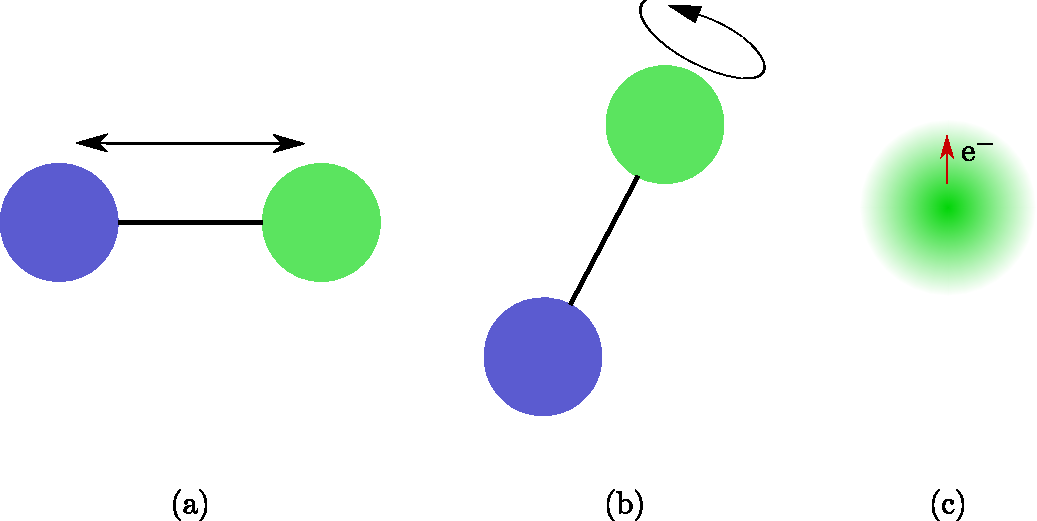
\includegraphics[width=0.5\linewidth]{figures/molecule_DOFs.pdf}
    \end{center}
    \caption{
    (a) Molecular vibration, (b) rotation, and (c) exciting an electron in an atom / molecule.
    }
    \label{fig:DOFs}
\end{figure}

The chemical bond is what forces atoms in a molecule to stay close enough together. If we were to try and take two atoms that are chemically bonded and rip them apart, we would be met with incredible resistance from the retaliation of the bond. On the flip side, there is a repulsive force between atoms that are bonded that ensures that the atoms don't get too close to each other. This balance between the repulsive and attractive forces determines the distance that separates atoms in a chemical bond (called \textit{bond length}). If we were to plot the potential energy stored in a molecule, $E_{bond}$, as a function of the two atoms' separation, $r$, it would look something like the blue or red curve in Fig.~\ref{fig:potential_curve}. It's at the very minimum point on the curves in Fig.~\ref{fig:potential_curve} where the attractive and repulsive forces are in equilibrium with each other.

\begin{figure}
    \begin{center}
        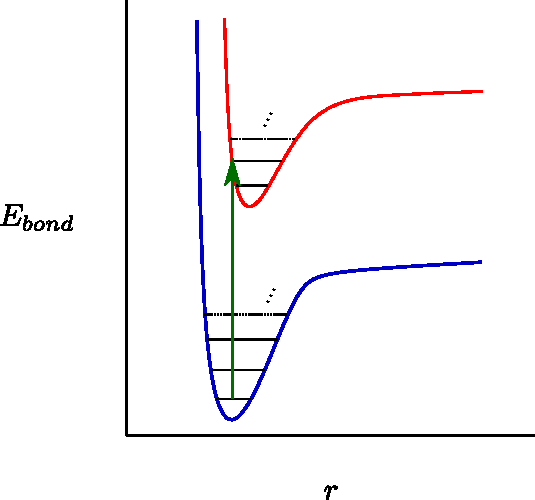
\includegraphics[width=0.4\linewidth]{figures/potential_energy_curve.pdf}
    \end{center}
    \caption{
    The general form of a molecule's potential energy curve as a function of bond length. The blue curve represents a molecule in its ground electronic state and the red curve represents the same molecule in an excited electronic state.
    }
    \label{fig:potential_curve}
\end{figure}

Vibrations affect the distance between the atoms, $r$, in the molecule. It turns out that the laws of quantum mechanics only allow for \textit{discrete} vibrational energies, and that the lowest vibrational energy that can be obtained (dubbed the ``ground'' vibrational state) is actually slightly above the minimum point on the blue/red curve. The allowed vibrational energy levels of the molecule are the horizontal lines within the blue curve in Fig.~\ref{fig:potential_curve}.

We can also think about exciting the molecule's electrons. If we were to do this, this can drastically change the interplay between the attractive and repulsive forces. Therefore, $E_{bond}$ as a function of $r$ changes significantly. The red and blue curves in Fig.~\ref{fig:potential_curve} are meant to represent the molecule in an excited electronic state and in its ground (lowest energy) electronic state, respectively. Note that the excited electronic state of the molecule also vibrates and therefore has its own discrete vibrational energy levels.

\subsubsection{Wavefunctions}

We need knowledge of one more thing before we can accomplish our goal of calculating Franck Condon Factors: wavefunctions. The wavefunction of a system, often denoted by the Greek letter $\psi$, is essentially the key to being able to calculate anything and everything about said system. In our spectroscopy language, the wavefunction of a molecule that we are interested in can be extremely complicated to fully determine. However, for our purposes we can ``separate'' the wavefunction of our molecule into parts describing its vibration ($v$), rotation ($R$) and electrons ($e$).
\begin{equation}
    \psi_{molecule} = \psi_e\psi_R\psi_v
\end{equation}

\subsubsection{Franck Condon Factors}

Armed with this conceptual knowledge of molecular vibrational energy levels and wavefunctions, we can now learn about Franck Condon Factors (FCFs). Picture the following scenario. We have a molecule in its ground state (both vibrationally and electronically), and we excite it electronically (i.e. move from the blue curve to the red curve in Fig.~\ref{fig:potential_curve}). To a very good approximation, it turns out that electronic transitions are so fast that the distance separating atoms in a molecule does not have time to adjust (this is the Franck Condon Principle). Diagrammatically, we are looking at the vertical green line in Fig.~\ref{fig:potential_curve} (it is vertical because the atoms in the molecule stays at the same distance apart during the transition). This specific ``vertical'' transition from the ground electronic and vibrational state to the excited electronic state and its second vibrational state will have a \textit{transition intensity} that is related to the vibrational part of the wavefunctions describing the system before and after the transition. More specifically, the transition intensity is proportional to the square \textit{overlap} (think of a vector dot product) between the two vibrational wavefunctions.
\begin{equation}
    \text{Transition}\text{ intensity} \propto \text{overlap}(\psi_{v,\text{before}},\psi_{v,\text{after}})^2
\end{equation}
The square of this overlap is precisely the Franck Condon Factor!
\begin{equation}
    \text{FCF} = \text{overlap}(\psi_{v,\text{before}},\psi_{v,\text{after}})^2
\end{equation}

\subsubsection{A simplified model for vibrations of diatomic molecules (2-atom molecules)}
One of the simplest ways to represent vibrations of diatomic molecules is to consider they are connected by a spring. The frequency of the vibration is a property of the molecule (and remains the same regardless of the energy the system has) and can be easily calculated using the masses of the atoms and the stiffness of the spring. This ``spring system'' is denoted a harmonic oscillator.

\begin{figure}
    \begin{center}
        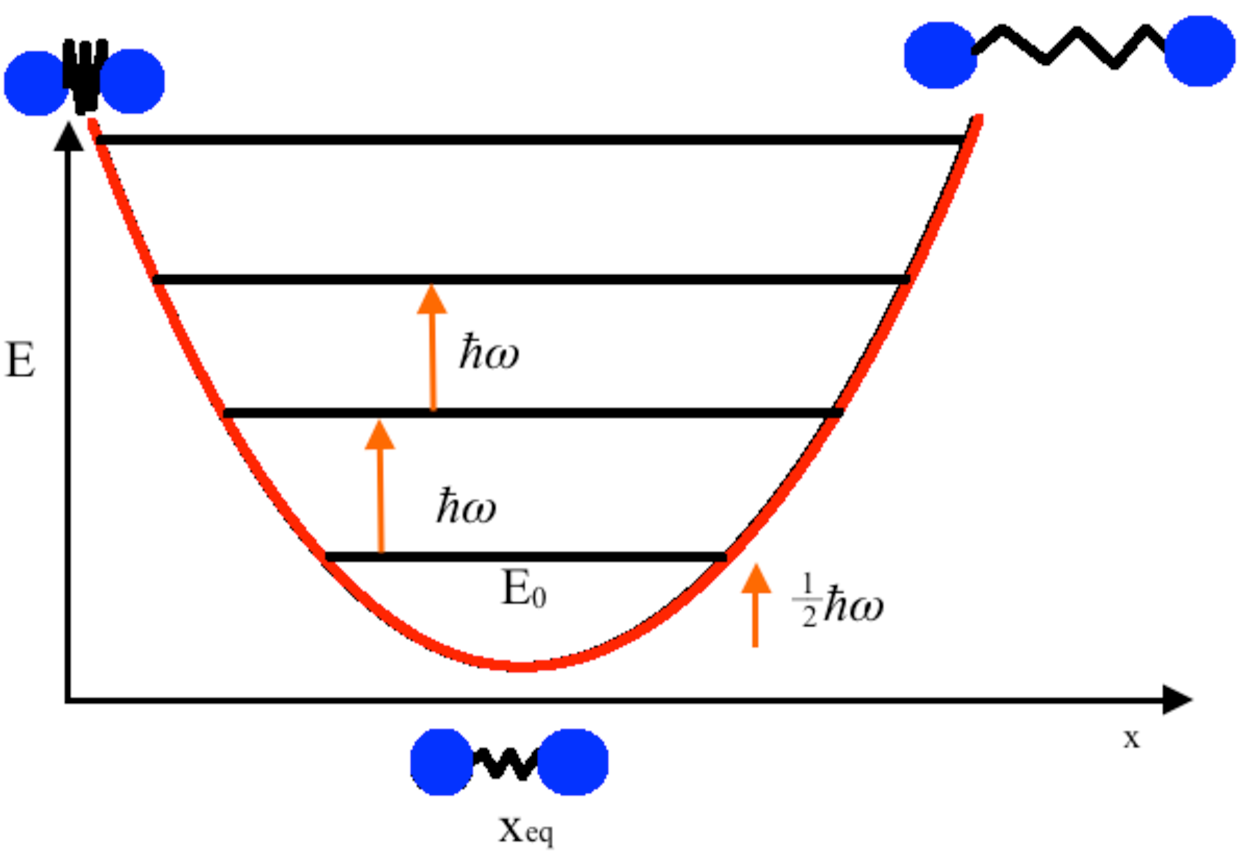
\includegraphics[width=0.4\linewidth]{figures/Harmonic_Oscillator.pdf}
    \end{center}
    \caption{
    A representation of a diatomic and it's vibrational energy levels in the harmonic oscillator approximation. The properties of this diatomic are it's equilibrium geometry, $x_{eq}$, it's frequency, $\omega$, and it's reduced mass, $\mu$. The ground state energy ($E_0$) is $\frac{1}{2}\hbar\omega$ from the potential minimum and vibrational energy differences between adjacent levels is $\hbar\omega$.
    }
    \label{fig:harmonic_curve}
\end{figure}

Refer to Fig.~\ref{fig:harmonic_curve} for the energy levels associated with a harmonic oscillator system. If a molecule is in it's ground vibrational state, it will ``stretch'' and ``contract" about it’s natural (or equilibrium) bond length. As it gains energy and moves into excited vibrational states, it can stretch and contract further and further from it’s equilibrium bond length, however it continues to vibrate at the same natural frequency.

The harmonic oscillator is a simplified model, since it ignores all repulsive effects of the 2 atoms within the molecule (the steep wall at small $r$ denoted by a more realistic potential energy curve in Fig.~\ref{fig:potential_curve}). As well, the harmonic oscillator potential has no dissociation (or bond-breaking) as is denoted by the flat portion at large $r$ in the potential energy curve in Fig.~\ref{fig:potential_curve} meaning at higher excited states, the atoms will continue to stretch further and further without the ``spring snapping.''
\newpage
However, the harmonic oscillator has a unique feature, in that the energy levels are equally spaced and the wavefunction takes an analytic form, allowing for simple calculations.

$\psi_n(x) = \frac{1}{\sqrt{2^nn!}}\cdot\left(\frac{\mu\omega}{\pi\hbar}\right)\cdot\exp\left(-\frac{\mu\omega (x-x_{eq})^2}{2\hbar}\right)\cdot H_n\left(\sqrt{\frac{\mu\omega}{\hbar}}(x-x_{eq})\right)$ , n=0,1,2,...

\noindent where $\mu$ is the reduced mass of the molecule, $\omega$ is it's vibrational frequency, $x$ is the bond length, $x_{eq}$ is the equilibrium bond length, $n$ is the vibrational state of the system, and $H_n$ is the Hermite polynomial.

\subsubsection{Project 1: Calculate Franck-Condon Factors for H$_2$-H$_2^+$ using the harmonic oscillator approximation}
You are provided with a Python code FCF-H2.py which calculates all of the information you require.

\noindent This code takes as input:
\begin{enumerate}
    \item Reduced mass of H$_2$ molecule (same as H$_2^+$)
    \item Frequency of the H$_2$ molecule
    \item Frequency of the H$_2^+$ molecule
    \item Difference in bond length (displacement)
    \item Difference between potential minima of the electronic states ($\Delta T_e = T_e^{'} - T_e$)
    \item Number of ground and excited vibrational states required for output
\end{enumerate}

\noindent This code outputs:
\begin{enumerate}
    \item Franck-Condon Factors for each pair of ground and excited vibrational states up to a threshold, using the n$_{H_2}$ = 0, n$_{H_2^+}$ = 0 Franck-Condon factor as the reference.
\end{enumerate}

\noindent Your task will be to determine the spectra of at least 10 transitions with a relative Franck-Condon factor greater than 1\%, where the FCF is the intensity and the spectral position is defined as:


Spectral Position = $\Delta T_e + E_{H_2^+} - E_{H_2}$

and expanded to:

Spectral Position = $\Delta T_e +\hbar\omega_{H_2^+}(n_{H_2^+} + \frac{1}{2}) - \hbar\omega_{H_2}(n_{H_2} + \frac{1}{2})$
\newpage

\subsection{Week 4: Ising Annealer}

\newpage

\bibliography{refs}
\bibliographystyle{unsrt}

\end{document}
